\documentclass[a4paper,10pt]{article}
\usepackage[margin=1in]{geometry}
\usepackage{lipsum}
\usepackage{graphicx, float}
\usepackage{xcolor}
\def\red#1{\textcolor{red}{#1}}


\begin{document}
\section*{\centering Point-by-point response to referee comments}

We thank the reviewers for taking the time to read over and give constructive feedback on our paper titled “\emph{Inverse energy transfer in three-dimensional quantum vortex flows}", submitted to PRL. Please see below the point-by-point response to the comments made by the reviewers.

\subsection*{Referee 1}

\begin{enumerate}
    \item The total helicity during the reconnection event is not conserved. The presence of the mutual friction force introduces a dissipation into the normal fluid. Overall, by computing the helicity in the superfluid component, we confirmed this. We decided to omit this plot from the manuscript so as to not introduce further concepts of superfluid helicity to a paper whose narrative is normal fluid centric. We have addressed the referees concern by inserting an additional statement to clarify that the helicity during the reconnection event is not in fact conserved. 
    \item The initial configuration is set up such that the superfluid velocity circlation in each half box has the opposite sign to the other half box, this is required to satisfy the periodic boundary conditions in the superfluid component. In the timescale of the simulation, we only observe one pair of the vortices which reconnect. During the reconnection, due to the large injection the helicity from the other pair is anyway negligible. The extended version of the simulation shows that the second reconnection injects positive helicity in the normal fluid, which then decays back to zero. Additionally, we computed the normal fluid helicity in each respective half box which also confirms this. We have added a sentence in the text to further clarify that the effect of the second vortex is negligent. \red{Add the new figure helicity\_normal\_fluid.pdf instead of Fig.2?}
    \item We appreciate the referee’s careful reading of the manuscript and their observation regarding a perceived inconsistency between the plots of the energy spectrum and the energy flux. Firstly, we would like to note the following points that should be considered:
    \begin{itemize}
        \item The energy spectrum is on a logarithmic scale - the energy flux is on a linear scale.
        \item The two plots are scaled differently: The energy spectrum is displayed in units of the code, while the energy flux is scaled by the energy flux at reconnection.
        \item The energy spectrum and energy flux don't have the same units.
    \end{itemize}
    We would like to clarify that what may appear as an inconsistency arises from the omission of the injection spectrum in the figures presented in the paper, which shows that the injection is larger postreconnection for $T=1.9$K.
    
    In the Navier-Stokes model that we employ, the rate of the energy spectrum is given by
    \begin{equation}
        \frac{\partial E(k)}{\partial t} = -\frac{\partial \Pi(k,t)}{\partial k} + D(k,t) + I(k,t)
    \end{equation}
    where $\Pi(k,t)$ represents the energy flux, $D(k,t)$ the dissipation spectrum and $I(k,t)$ the injectrum spectrum, resulting from the mutual fricition force. The injection spectrum was not included in the manuscript for brevity but is fully consistent with the presented data.

    \begin{figure}[H]
        \centering
        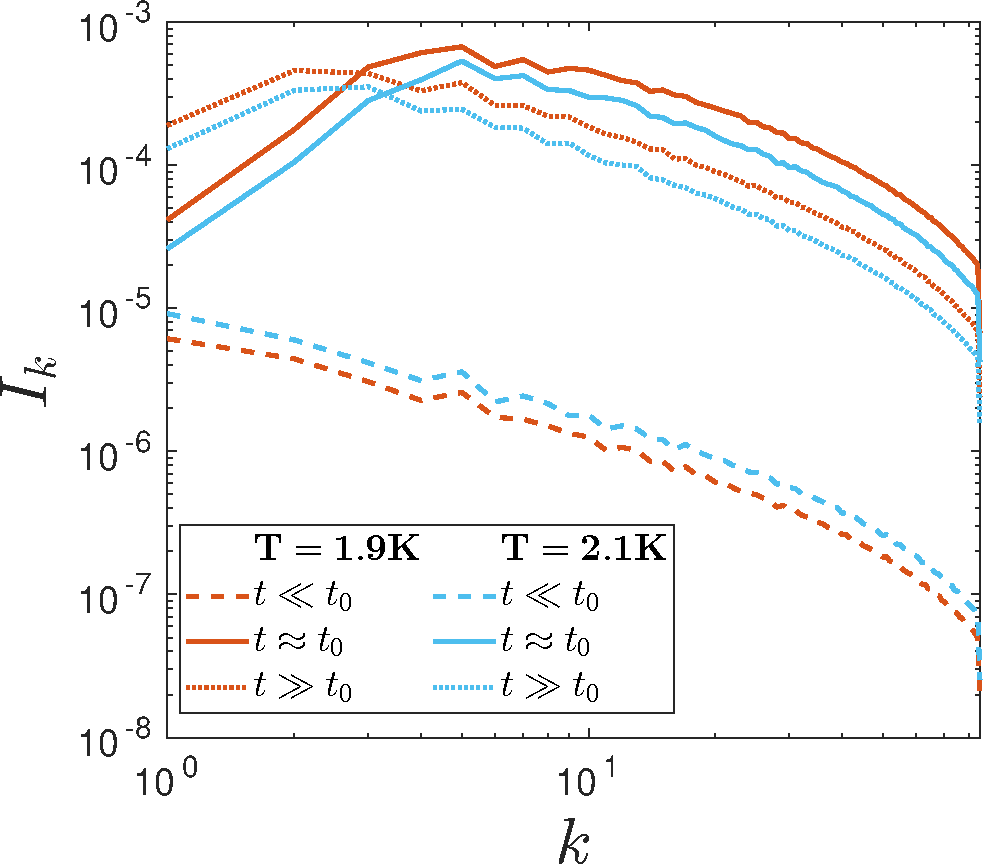
\includegraphics[width=0.4\textwidth]{inj-spec.pdf}
    \end{figure}

    To clarify this point, we have included a supplementary figure showing the injection spectrum, which demonstrates how it complements the energy flux and spectrum, thereby resolving the apparent discrepancy. We have also updated Fig.3a to ensure consistency with the scaling used throughout the manuscript.    
    %We will also include a brief explanatory note in the revised manuscript to ensure this is clear to readers.



    \item 
    \item The value $t_0$ should in fact be $t_R$, the typo has been corrected.
    \item The authors agree with the comment of the referee that the current notation is not ideal. Instead, the figures have been changed to use the timescale in the horizontal axis of all time plots. Additionally to note, we have replaced the vertical axis label of Fig. 3b with $E_R/\tau_R$, simply a change of symbols to make clear the non-dimensionalisation of units.
    \item The figure has been updated with a power law of $k^{-3}$ 
    \item The time $t^*$ was introduced as the time at which we observe a sufficient decay of the helical force ratio, where the difference is around 5\% between the positive and negative modes and remains relatively stable afterwards. In order to make this clearer, we have added a sente nce in the text to explicity state this.
    \item The value of 0.1s comes from dimensionalising the values of $\tau=0.01$ for $T=1.9K$ and $\tau=0.005$ for $T=2.1K$, using the values of $\tilde{\tau}$ listed in the supplementary materials. 
    \item Incorrect reference corrected as noted by the reviewer.
\end{enumerate}

\subsection*{Referee 2}

\end{document}
